%%%%%%%%%%%%%%%%%%%%%%%%%%%%%%%%%%%%%%%%%%%%%%%%%%%%%%%%%%%%%%%%%%%%%%%%
% 4. エレベータ利用者の行動パターンと待ち時間の推定
%%%%%%%%%%%%%%%%%%%%%%%%%%%%%%%%%%%%%%%%%%%%%%%%%%%%%%%%%%%%%%%%%%%%%%%%

\section{Behavior patterns of people using elevators and estimation of waiting time}
In this chapter, we describe a method to estimate the behavior pattern and waiting time of elevator users based on the time-series RSSI data of BLE signals obtained from the system described in the previous chapter. 

% 図:時系列RSSIデータ
\begin{figure}[t]
\centering
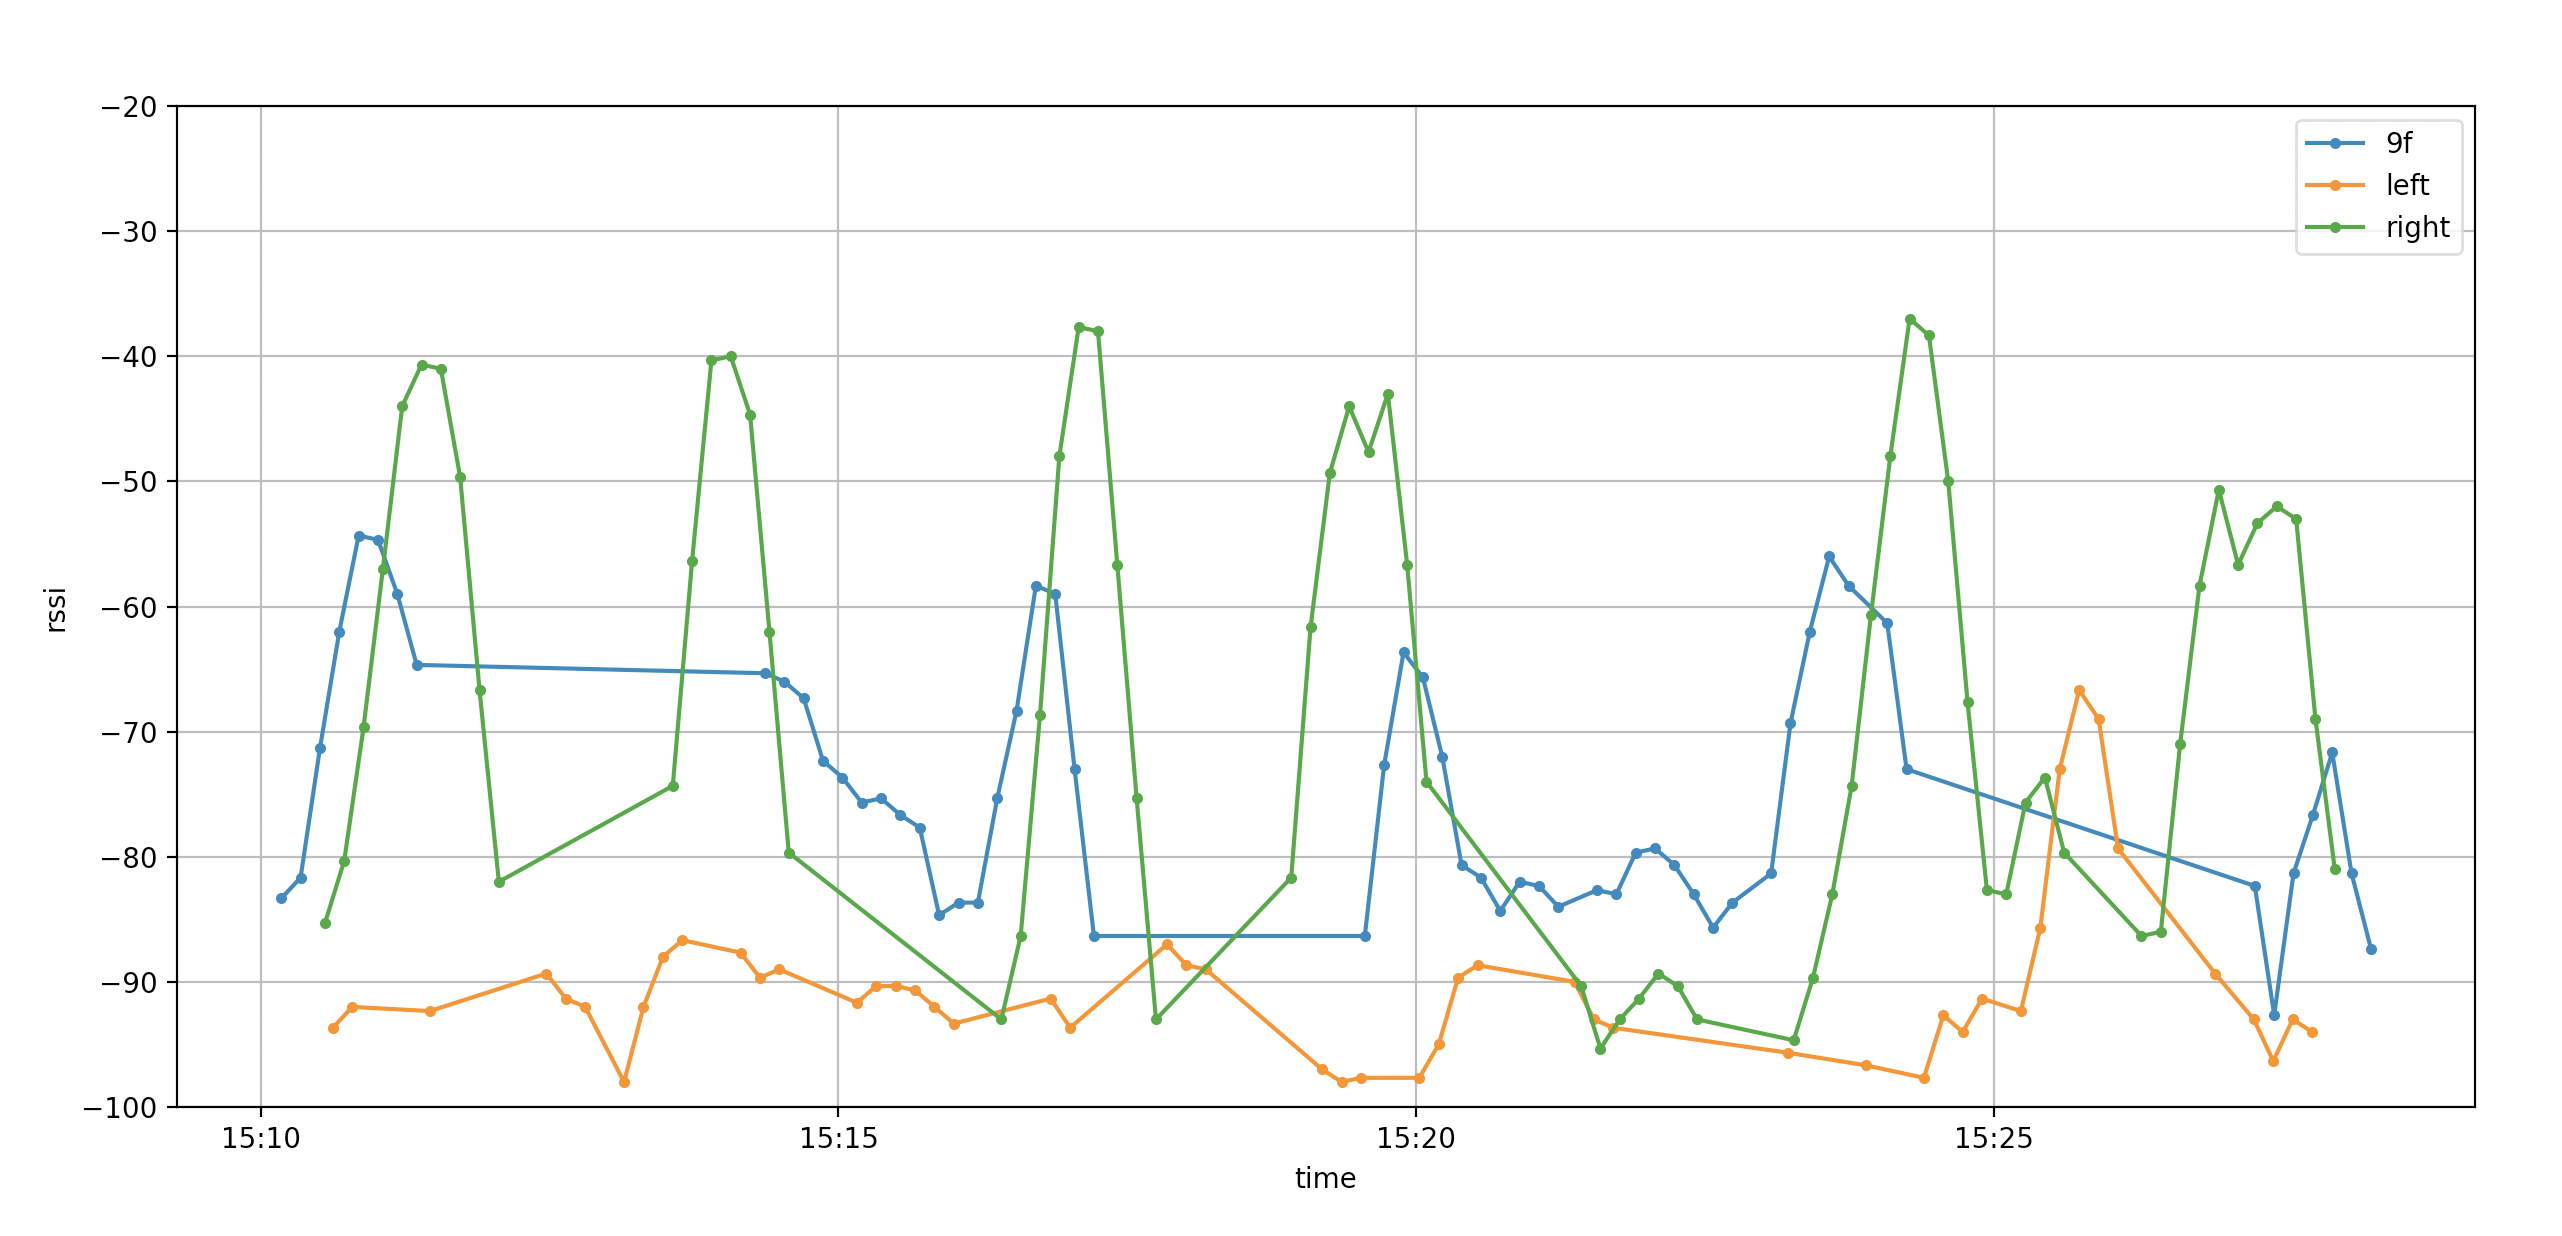
\includegraphics[width=1.0\hsize]{img/ble_rssi_original.png}
\caption{Time series RSSI data}
\label{fig:ble_rssi_original}
\end{figure}

% 対象とするエレベータ利用者の行動パターン
\subsection{Behavioral patterns of people who use the target elevators}

The following four types of behavioral patterns of elevator users are targeted in this study.

\begin{quote}
 \begin{itemize}
  \item Board the elevator.
  \item Exit the elevator.
  \item Use stairs instead of elevators.
  \item Passing in front of the elevator.
 \end{itemize}
\end{quote}

% 行動パターンと待ち時間を推定するアルゴリズム
\subsection{Algorithm for estimating behavior patterns and waiting times}
This section describes an algorithm for estimating the activity pattern described in 4.1 from time-series RSSI data.
Let $A_{hall}$, $A_{right}$, and $A_{left}$ be the time-series RSSI data acquired from the tablet installed in front of the elevator hall, the smartphone installed in the elevator on the right, and the smartphone installed in the elevator on the left, respectively. In $A_{hall}$, $T_{start}$ is the time when the RSSI value reaches -70 dBm or higher. Let $T_{end}$ be the time when the RSSI value drops more than 10 dBm from the maximum value. Let the time 10 seconds before $T_{start}$ be $T_{start}'$ and the time 10 seconds after $T_{end}$ be $T_{end}'$, and let the data of $A_{right}$ and $A_{left}$ from $T_{start}'$ to $T_{end}'$ be $A_{right}'$ and $A_{left}'$. If the maximum RSSI values of $A_{right}'$ and $A_{left}'$ are both below -70 dBm, it is judged that ''Use stairs instead of elevators'' or ''Passing in front of the elevator''. If the maximum value of RSSI of $A_{right}'$ is higher than that of $A_{left}'$, it is judged as ''boarded the elevator on the right side'' or ''got off from the elevator on the right side'', and if it is lower than that, it is judged as ''boarded the elevator on the left side'' or ''got off from the elevator on the left side''. If the time at which the RSSI value of $A_{right}'$ reaches the maximum is later than the time at which the RSSI value of $A_{hall}$ reaches the maximum, it is judged to be ''boarding the right elevator'', and if it is earlier, it is judged to be ''getting off from the right elevator''. The same procedure is applied to ''getting on the left elevator'' or ''getting off from the left elevator''. In the case of ''getting on the elevator'', the difference between $T_{start}$ and $T_{end}$ is regarded as the waiting time.


% 実験方法
\subsection{Experimental Methods}

The experiment is conducted in the elevator on the 9th floor of the West 2 Building of Kyushu University, Ito Campus (Figure \ref{fig:kyudai_west2_elevator}). In this experiment, two kinds of behavioral patterns, ''getting on the elevator on the right side'' and ''getting off the elevator on the right side'', were reproduced and tested with an iPhone with COCOA installed. The experimental method is described below.

First, the participants pushed the ''get off'' button in front of the elevator hall on the 9th floor and waited in front of the elevator on the right side until the elevator arrived. Get on the elevator, move to the first floor, and get off the elevator. After waiting for a minute or two, press the ascending button in front of the elevator hall on the first floor and follow the same procedure to the ninth floor. Repeat this procedure for three sets. Record the time you press the elevator button, the time you get on the elevator, and the time you get off the elevator (\tablename\ref{table:record_table}).


% 実験結果
\subsection{Experimental results}

The time series RSSI data from 15:10:00 to 15:30:00 obtained from the tablet terminals in front of the elevator hall on the 9th floor and the smartphone terminals installed in the elevators on the right and left sides are shown in Figure \ref{fig:ble_rssi_original}.
Based on the algorithm, the detection rate of boarding and alighting was 100\%. The estimated waiting time on the 9th floor when a passenger gets on the train is shown in Figure \ref{fig:ble_rssi_9f_wait}, Figure \ref{fig:ble_rssi_9f_wait_quess} and \tablename\ref{table:record_table_guess}. Compared to \tablename\ref{table:record_table}, the estimated wait times are roughly consistent, although there may be a time lag of 5 to 10 seconds between the estimated start time ($T_{start}$) and estimated end time ($T_{end}$). Currently, the timing of the BLE scan is assumed to be about once every 10 seconds, but if the interval of the scan is shortened, the accuracy is expected to be improved.

% 表:実験の記録
\begin{table*}[ht]
\caption{Record of the experiment}
\label{table:record_table}
\begin{tabular}{c|ccc|c}
\hline
\textbf{\begin{tabular}{c}behavioral \\ pattern\end{tabular}} & 
\textbf{\begin{tabular}{c}Time when \\ the elevator button \\ is pressed\end{tabular}} & 
\textbf{\begin{tabular}{c}Time of \\ the elevator \\ ride\end{tabular}} & 
\textbf{\begin{tabular}{c}Time \\ you got off \\ the elevator\end{tabular}} & 
\textbf{\begin{tabular}{c}waiting \\ time\end{tabular}} \\
\hline\hline
Move from 9F to 1F & 15:10:31 & 15:11:01 & 15:11:22 & 30sec \\
Move from 1F to 9F & 15:13:20 & 15:13:45 & 15:14:10 & 25sec \\
Move from 9F to 1F & 15:16:32 & 15:16:50 & 15:17:22 & 18sec \\
Move from 1F to 9F & 15:19:00 & 15:19:12 & 15:19:43 & 12sec \\
Move from 9F to 1F & 15:23:17 & 15:23:58 & 15:24:34 & 41sec \\
Move from 1F to 9F & 15:25:55 & 15:26:42 & 15:27:32 & 47sec \\
\hline
\end{tabular}
\end{table*}

% 図:時系列RSSIデータと9Fでの待ち時間
\begin{figure}[t]
\centering
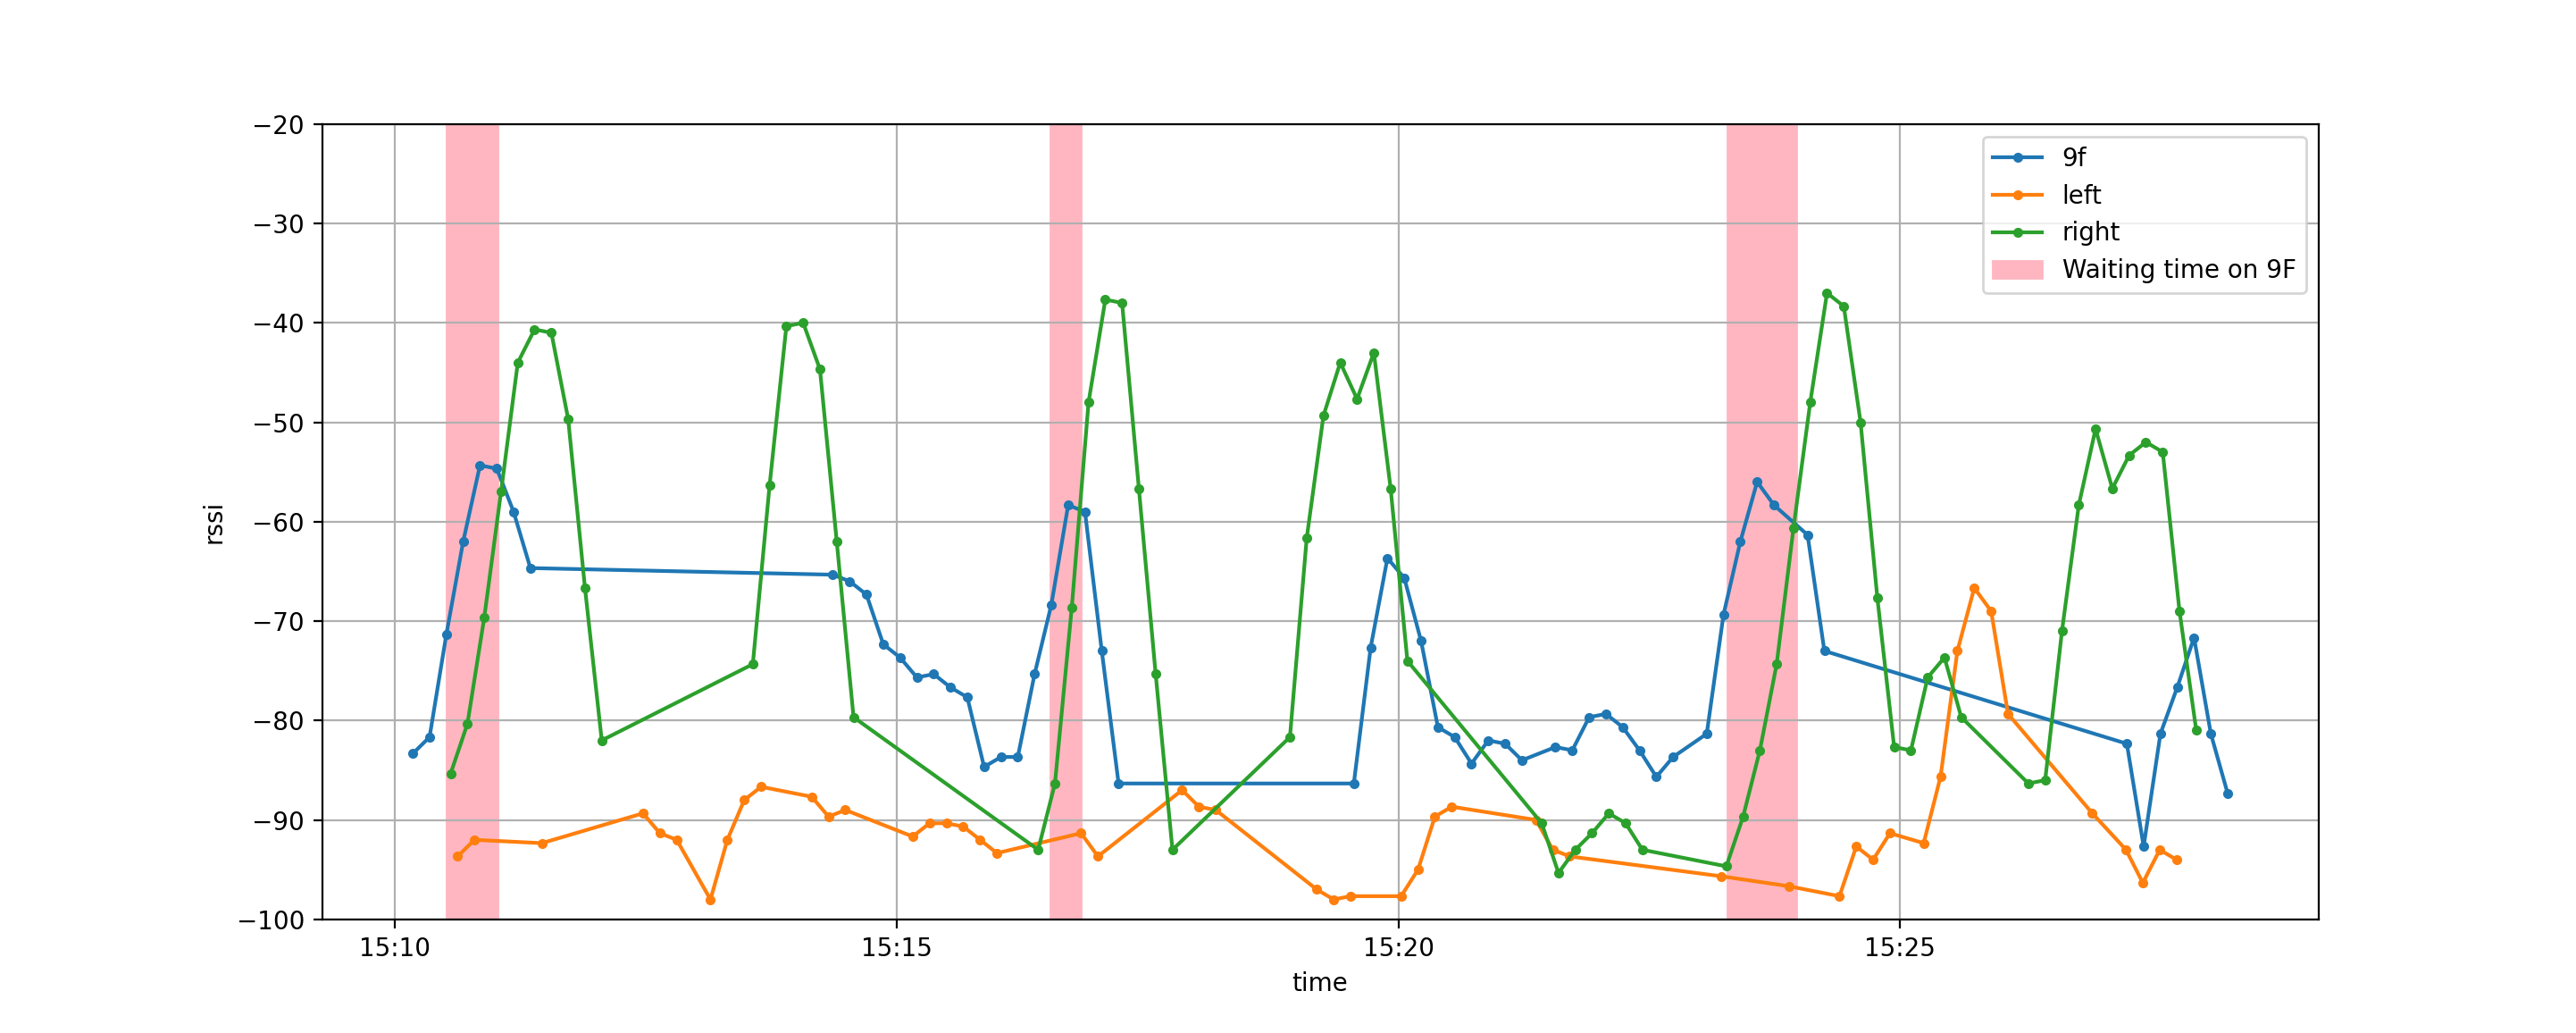
\includegraphics[width=1.0\hsize]{img/ble_rssi_9f_wait.png}
\caption{Time series RSSI data and waiting time at 9F and Actual waiting time}
\label{fig:ble_rssi_9f_wait}
\end{figure}

% 図:時系列RSSIデータと9Fでの待ち時間(推定値)
\begin{figure}[t]
\centering
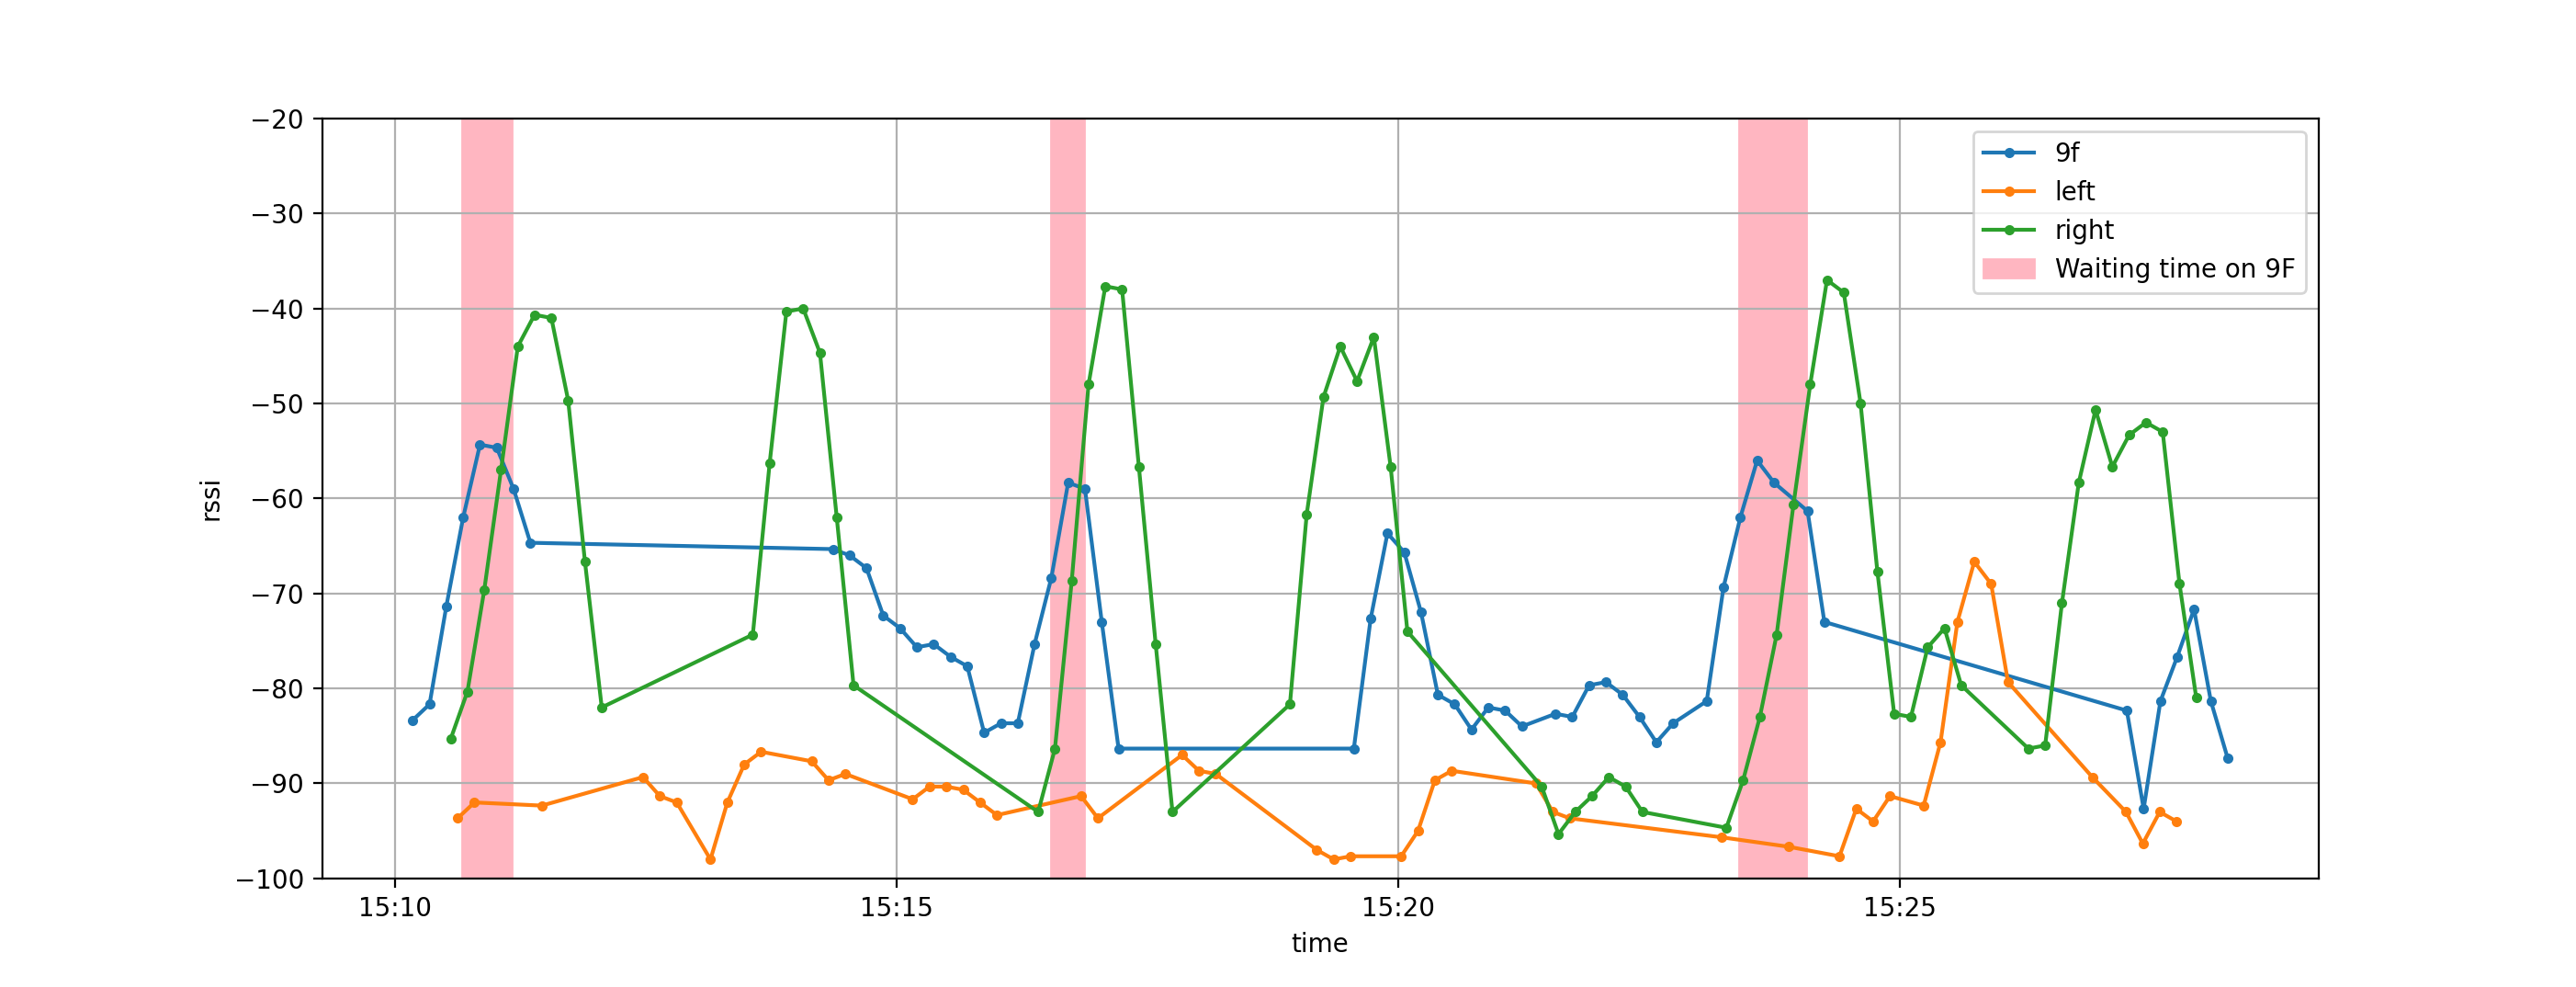
\includegraphics[width=1.0\hsize]{img/ble_rssi_9f_wait_guess.png}
\caption{Time series RSSI data and waiting time at 9F and Estimated latency by algorithm}
\label{fig:ble_rssi_9f_wait_quess}
\end{figure}

% 表:アルゴリズムによる推定待ち時間
\begin{table*}[ht]
\caption{Estimated latency by algorithm}
\label{table:record_table_guess}
\centering
\begin{tabular}{c|cc|c}
\hline
\textbf{behavioral pattern} & \textbf{$T_{start}$}  & \textbf{$T_{end}$} & \textbf{Estimated waiting time} \\ \hline\hline
Take the right elevator. & 15:10:40 & 15:11:10 & 30sec \\
Take the right elevator. & 15:16:32 & 15:16:52 & 20sec \\
Take the right elevator. & 15:23:24 & 15:24:04 & 40sec \\
\hline
\end{tabular}
\end{table*}
